\documentclass[conference]{IEEEtran}
\IEEEoverridecommandlockouts
% The preceding line is only needed to identify funding in the first footnote. If that is unneeded, please comment it out.
\usepackage{cite}
\usepackage{array}
\usepackage{listings}
\usepackage{amsmath,amssymb,amsfonts}
\usepackage{algorithmic}
\usepackage{hyperref}
\usepackage{graphicx}
\usepackage{textcomp}
\usepackage{xcolor}
\def\BibTeX{{\rm B\kern-.05em{\sc i\kern-.025em b}\kern-.08em
    T\kern-.1667em\lower.7ex\hbox{E}\kern-.125emX}}
\begin{document}

\title{6 things must to do\\
{\footnotesize \textsuperscript{}Break manerism by ivy lee method}
\thanks{Identify applicable funding agency here. If none, delete this.}
}

\author{\IEEEauthorblockN{Changhoi Kim}
\IEEEauthorblockA{\textit{Dept. of Information System} \\
\textit{Hanyang Univ}\\
Seoul, Korea \\
changhoi0522@hanyang.ac.kr }
\and
\IEEEauthorblockN{Jungeun Kim}
\IEEEauthorblockA{\textit{Dept. of Information System} \\
\textit{Hanyang Univ}\\
Seoul, Korea \\
wjddms04@hanyang.ac.kr }
\and
\IEEEauthorblockN{Eunchai Kim}
\IEEEauthorblockA{\textit{Dept. of Information System} \\
\textit{Hanyang Univ}\\
Seoul, Korea \\
eunchai512@naver.com }
}

\maketitle

\begin{abstract}
“6 things must to do” is an application that helps people practice Ivy Lee Method, a way to get rid of mannerisms and manage time efficiently. We use artificial intelligence speaker NUGU to help users set up 6 things each day and manage tasks to be done every day
\end{abstract}
\begin{IEEEkeywords}
ivy lee method,  6 things, mannerism, nugu, ai speaker, todo list
\end{IEEEkeywords}

\begin{table}
\caption{Role Assignments}
\begin{center}
\begin{tabular}{ | m{4em} | m{2cm}| m{4cm} | }
\hline
\textbf{\textit{Role}}& \textbf{\textit{Name}}& \textbf{\textit{Task}} \\
\hline
User& NUGU Speaker and Application user & Application can use for free on IOS and AOS. Every NUGU Speaker and application users can use default feature of application. \\
\hline\
Customer& SKT and Application User & Customer want to solve the problems at an acceptable cost . SKT want application which is running on NUGU speaker, so more NUGU users get advantages. Application users who want more advanced feature of application will pay subscription fee. \\
\hline
Software Developer & Changhoi Kim, Jungeun Kim & Engineers create actual product. They demand core function requirements, which give then up to their developing process, to manager. Software developers’ goal is to satisfy users and customers by realizing close to the requirements. \\
\hline
Development Manager & Eunchai Kim & Development managers intercommunicate with Customer and Software developer to satisfy with whole stakeholders. They schedule timeline to stick to the project before deadline. They also build overall developing process and support software developers.\\
\hline
\end{tabular}
\label{tab1}
\end{center}
\end{table}

\section{Introduction}
Ivy Lee Method is a technology for efficient time management used over a long period of time. It is proposed by Ivy Lee to executives and employees to eliminate corporate manners and improve productivity. Next are the following the five steps:\\

\begin{enumerate}
\item Set up six things to do for next day before bed. \\
\item Arrange in the order of priority among the six things. \\
\item The things are executed according to the priority set, and the next thing cannot be carried out until the previous thing is completed. \\
\item If the assignment is not completed, the remaining tasks will be carried out the next day. \\
\item Repeat the above method every day. \\
\end{enumerate}
 
This method makes modern people, surrounded with many tasks, think of the most important ones to be carried out. Since the method is simple enough for anybody to follow, it can be implemented until the execution stage. Also to eliminate the fear of starting from scratch. Furthermore, this helps break down mannerism and create a productive day. \\
 
The most complete application derived from the existing Ivy Lee Method was the application called “6 things”. This application is a To-Do list app that writes down six things to do. However, it does not force a priority, but rather only writes down six To-Do list. Also it does not store the degree of achievement of other days. Moreover, record cannot be checked, feedbacks cannot be made and no retrospection. \\

“6 things must to do” sends an alarm so that people can set the day or the next day task. Also sets the To-Do list and checks the list of achievement through the AI speaker NUGU. Using NUGU, people can also check the next thing to be completed or task that was completed. Through subscription services, we provide a dashboard to store daily records and check weekly and monthly attainment rates.\\

\section{Requirements}

\subsection{Mobile Application}

Mobile applications will be used by users. Both Android and iOS are available. Cross Platform applications to communicate with the server is required. There will be five four functions(login, task list, dashboard, social) in the application.\\

\begin{enumerate}
    \item Login: Users only use social login. So there are no local application login form. And there are no sign-up screen because the application will use the information which is from social login. There will be only simple login screen.
    \begin{enumerate}
        \item Additional information screen: Social login might give email and unique app id value. But if user refuses to provide an email and the user is new client, the user should type email manually for using application.\\
    \end{enumerate}
    \item Navigation tab: The Application has some features, so it need the navigation bar for split the domain. It is on the bottom of the screen.\\
    \item Tasks (Main Screen): Six tasks screen will be on the main screen. In addition to the task designation, various works will be available.
    \begin{enumerate}
        \item One task component: There is task component which shows the detail of one task.
        \begin{enumerate}
            \item Read tasks detail: By default, the component shows the detail of one task. it has "when", "where", "with whom" fields, and simple to-do list to complete the task.
            \item Set details of task: In this component, user can make detail of the task. The detail fields are as mentioned above.
            \item Update to-do status in a task: Each to-do in the to-do list of a task can be completed. When all the to-dos are completed, the task is completed, too. However if there are no detail to-do, user can complete the task by other button in detail component or in list component. \\
        \end{enumerate}
        \item Task list component: There is task list component which has plural task components.
        \begin{enumerate}
            \item Read task list of specific date: In this screen, the component shows the list of tasks. It is default screen of task list component.
            \item Add task: In task list screen, user can add task for next day (or next session of task list). The added task is consist of task component.
            \item Start tasks and lock the list: When user click lock button, the list become uneditable except complete the task. Lock time is set by user in settings screen.
            \item Check ongoing task and complete the task: When the task list is locked, user can find what task should be handled, and check the task as complete. If the task has specific to-do list, and user check the task as complete, all to-dos in the task is also checked as complete.
            \item Pass the remain incomplete tasks to next task list: When the session (user-set lock time) is over, and the list has remain tasks, The remaining list goes into the next (session's) task list.\\
        \end{enumerate}
        \item Dashboard: User can check the usage of the application in this component. There are graph for visualizing monthly, weekly, daily task processing degree. And also check the list of the specific date.\\
    \end{enumerate}
    
    \item Social: Users can find their own ranks on the list. The list shows the ranking of the users' friends or the world ranking, which is a ranking of every user who uses our app. It can add new friends to the list and share users' results of six tasks to the others. Also, search for other users and look for their result is available. \\
    \item Settings: User can set the option of the application. They can adjust alarm, Task list session time (Lock time), and change their account information in this component.\\

\end{enumerate}

\subsection{NUGU Service}

Also, user can access the application through NUGU AI speaker. User speak specific command and the NUGU speaker response and process the command. \\

\begin{enumerate}
    \item Check ongoing task: User can complete the task which is currently in progress. \\
    \item Complete the task: User can complete ongoing task \\
    \item Check the remain tasks: User can check the remain tasks in the list. \\
\end{enumerate}

\section{Development Environment}


\subsection{Choice of software development platform}

\begin{enumerate}
    \item Which platform and why \\
    Our service operates mainly on mobile applications. We use Cross Platform application that is available for both Android and iOS operating systems and we develop app focusing on the latest version due to development environmental limitations and time constraints. We are using React Native since it can develop both platforms. Our app is an app service based, not the web, because it needs to have easy access to the tasks and provide alarm service to the specific ones. \\
    
    The server application will work on Linux based Lambda of AWS. DynamoDB on AWS will be used for database. Lambda and DynamoDB can save the cost while building simple applications because of its generous free tier. \\
    
    We do not have to worry about infrastructure and can focus on server application logic when we use managed services of AWS like DynamoDB and Lambda. In addition, we think that golang is a suitable language to operate in Lambda system since it remains simple executable binary after compilation and does not have to run virtual machine like JVM.\\
    
    \item Which programming language and why
    \begin{enumerate}
        \item Typescript \\
        Typescript, Javascript's superset, provides more stable development environment. By defining the interface and types, errors caused by misusing the type are prevented in advance. It can also easily identify the specific way of using methods and functions. In addition to the above advantages, it is freely available to use the large open source system of JavaScript.\\
        \item Go \\
        Go language is a compile language, that has fast performance as C language. There is no complicated grammar, and by unifying some of the code styles, it reduces the concern about the convention. By using the computing power efficiently, relatively little computing resources are required to achieve the same goal as other languages.\\
        
        \item Finally, both languages are growing rapidly in terms of language utilization, especially typescript is becoming the standard for JS development environments. Golang also has a huge growing community and is in line with recent technology trends.\\
    \end{enumerate}
    \item Provide a cost estimation for your built \\
    
    \begin{table}[h!]
    \caption{Cost estimation}
    \begin{center}
    \begin{tabular}{ | m{6cm} | m{2cm} | }
    \hline
    \textbf{\textit{Name of software / hardware}}& \textbf{\textit{Cost}} \\
    \hline
    Apple Developer Program & 129,000 won \\
    \hline\
    AWS Lambda & 0 dollar \\
    \hline
    AWS DynamoDB & 0 - 5 dollar \\
    \hline
    \end{tabular}
    \label{tab1}
    \end{center}
    \end{table}
    \item Provide clear information of your development environment
    \begin{itemize}
        \item MacOS Catalina 10.15.7
        \begin{itemize}
            \item 2.3 GHz 8 Core intel Core i9 
            \item 32GB 2667 MHz DDR4 Memory 
        \end{itemize}
        \item Windows 10
        \begin{itemize}
            \item 1.80 GHz 8 Core Intel i7
            \item 8GB Memory
        \end{itemize}
        \item Visual Studio Code 1.50.1
        \item Goland 11.0.8 (2020.2)
        \item Go 1.15
        \item Gin 1.6.3
        \item Node 12.18.3
        \item Typescript 4.0.3
        \item React Native 0.63.3
        \item Git 2.28.0 
        \item Other open sources
            \begin{itemize}
                \item \href{https://github.com/6-things-must-to-do/app/blob/develop/package.json}{\textbf{Link: Open source used in mobile application}}
                \item \href{https://github.com/6-things-must-to-do/backend/blob/develop/go.mod}{\textbf{Link: Open source used in the server}}
            \end{itemize}
    \end{itemize}
    \item Using any commercial cloud platform \\
    
    AWS Lambda and DynamoDB will be used to launch production servers.  Computing and Database resources are the same information written above, and AWS API Gateway service will be used to proxy HTTP requests to Lambda. \\
    
\end{enumerate}




\subsection{Software in use}
\begin{enumerate}
    \item Git \\
    Git is a distributed version-control system for tracking changes in source code during software development. It manage the code version and make co-working with other programmer more easier. There is branch system which is core of co-working in git-managed source code with many engineer. Each developer write code for different features and then, the codes can be merged easily by git. \\
    
    \item Github \\
    GitHub is an American multinational corporation that provides hosting for software development and version control using Git. It has features about git and also has own feature about source access control. Source code can be managed by permission in github. \\
    
    \item Golang and Gin \\
    Golang is a statically typed, compiled programming language designed at Google. Golang is known as fast as C and maintainable as JAVA. It is compilable language and when it is compiled, a single binary file is created. The binary file can excutable in various platform (Go build command has OS option which is about what platform the binary will be excuted in). \\
    Gin is go web framework. It's full name is gin-gonic. It helps engineer to build web application server easily. It is opensource and maintained by many contributers. \\
    
    \item AWS \\
    AWS stands for amazon web service, which provides cloud computer. AWS has many availability zone, so engineer can build safe and solid application. AWS provides various computing type, and there are many managed services. Managed service means that engineers do not have to concern about infrastructure. AWS ensures that the service logic will work. That services like Lambda, DynamoDB, etc is called AWS serverless services that make developer to focus to build application, not infratructure. \\
    
    \item Typescript \\
    Typescript is superset of javascript. Javascript is not type-safety language, so using javascript in huge project can make dangerous bug. Typescript can be used in javascript project, and also only typescript project. It is opensource and has huge engineer commnunity and maintained by Microsoft. \\
    
    \item React Native \\
    React Native is framework for mobile cross platform. This framework is created by Facebook. It works on Typescript and Javascript environment. TS/JS code create Native code which is written in JAVA (Android) and Objective-C(iOS).
    
\end{enumerate}

\subsection{Task distribution}

\begin{table}[h!]
\caption{Task distribution}
\begin{center}
\begin{tabular}{ | m{2cm} | m{6cm} | }
\hline
\textbf{\textit{Name}}& \textbf{\textit{Task Distribution}} \\
\hline
Changhoi Kim& Build servers, including databases, and manage the whole project (Server, DB) \\
\hline\
Jungeun Kim & Connect the server and the mobile app, and the data values received from the server (Redux, Container) \\
\hline
Eunchai Kim & Align the received data and design UI and CSS (Screen) \\
\hline
\end{tabular}
\label{tab1}
\end{center}
\end{table}

Our roles were distributed by technology rather than by app function. Our app has multiple functions, and we tried to divide the roles by the functions (ex. Making tasks/ Managing tasks/ Adding friends). However, we found out this method is inefficient, and it would be difficult to complete the project if we proceed it this way. It is because we realized that it is almost impossible to learn all the different skills to create a single function in time. Therefore, we eventually decided to divide the tasks by component of the app rather than the function, and let each person take charge of it. \\

\section{Specifications}
\subsection{Mobile Application}

\begin{figure}[htp] \centering 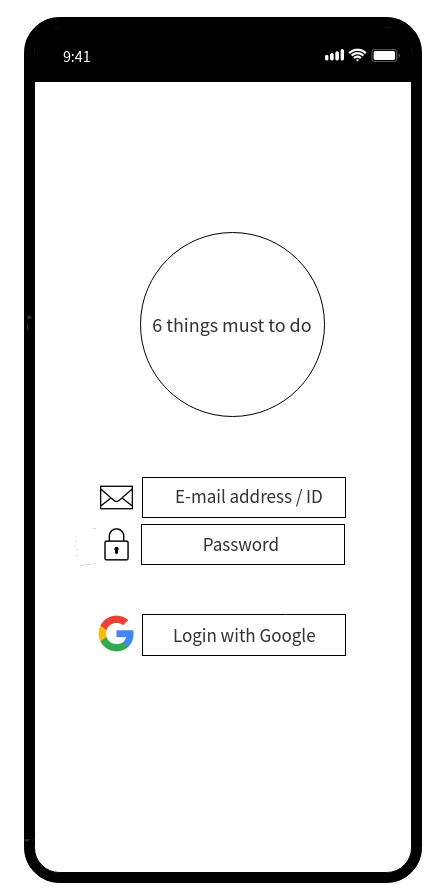
\includegraphics[width=120pt]{mockup_login} \caption{Login Screen} \label{fig:login} \end{figure}

\begin{enumerate}
    \item Login: \\
    Our application only has Google login. There are no other processes for signing up or signing in. Social login provides email, and unique app Id, etc. Using this information, application gets token from api server, and saves it in the device local storage. In the server, it takes social account information and gets user data in DynamoDB or creates user, then JWT which is to be used when user accesses api service.
    \begin{lstlisting}[frame=single]
    # in Application
    socialAccount := googlaLogin()
    token := getToken(socialAccount)
    saveTokenInLocalStorage(token)
    \end{lstlisting}
    
    \begin{lstlisting}[frame=single]
    # in API Server
    socialData := getRequest()
    user := getUserOrCreate(socialData)
    token := issueToken(user)
    response(token)
    \end{lstlisting}
 
\begin{figure}[htp] \centering 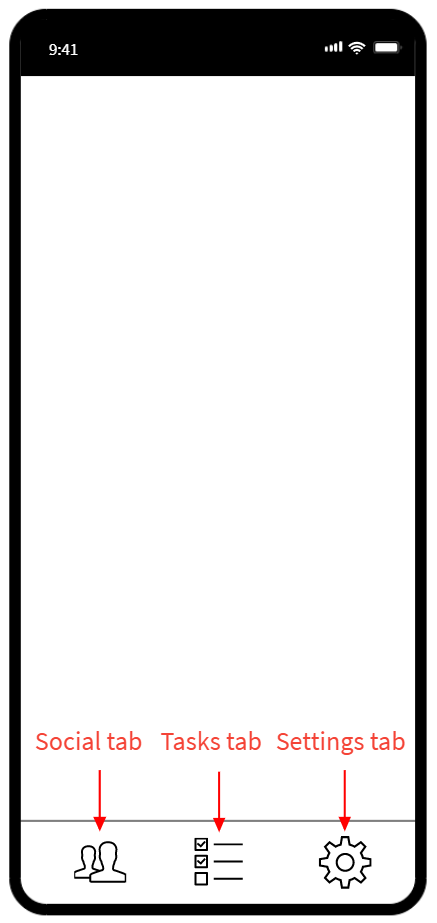
\includegraphics[width=120pt]{2) Navigation bar.PNG} \caption{Navigation tab} \label{fig:Navigation tab} \end{figure}
   
    \item Navigation tab: \\ 
    Navigation tab on the bottom of the screen includes social, tasks, settings tabs and is provided by open source named React Navigation. There is no other Network I/O.
    \begin{lstlisting}[frame=single]
    onChangeTab(targetScreen) {
        currentScreen = targetScreen
        re-render()
    }
    \end{lstlisting}
    
\begin{figure}[htp] \centering 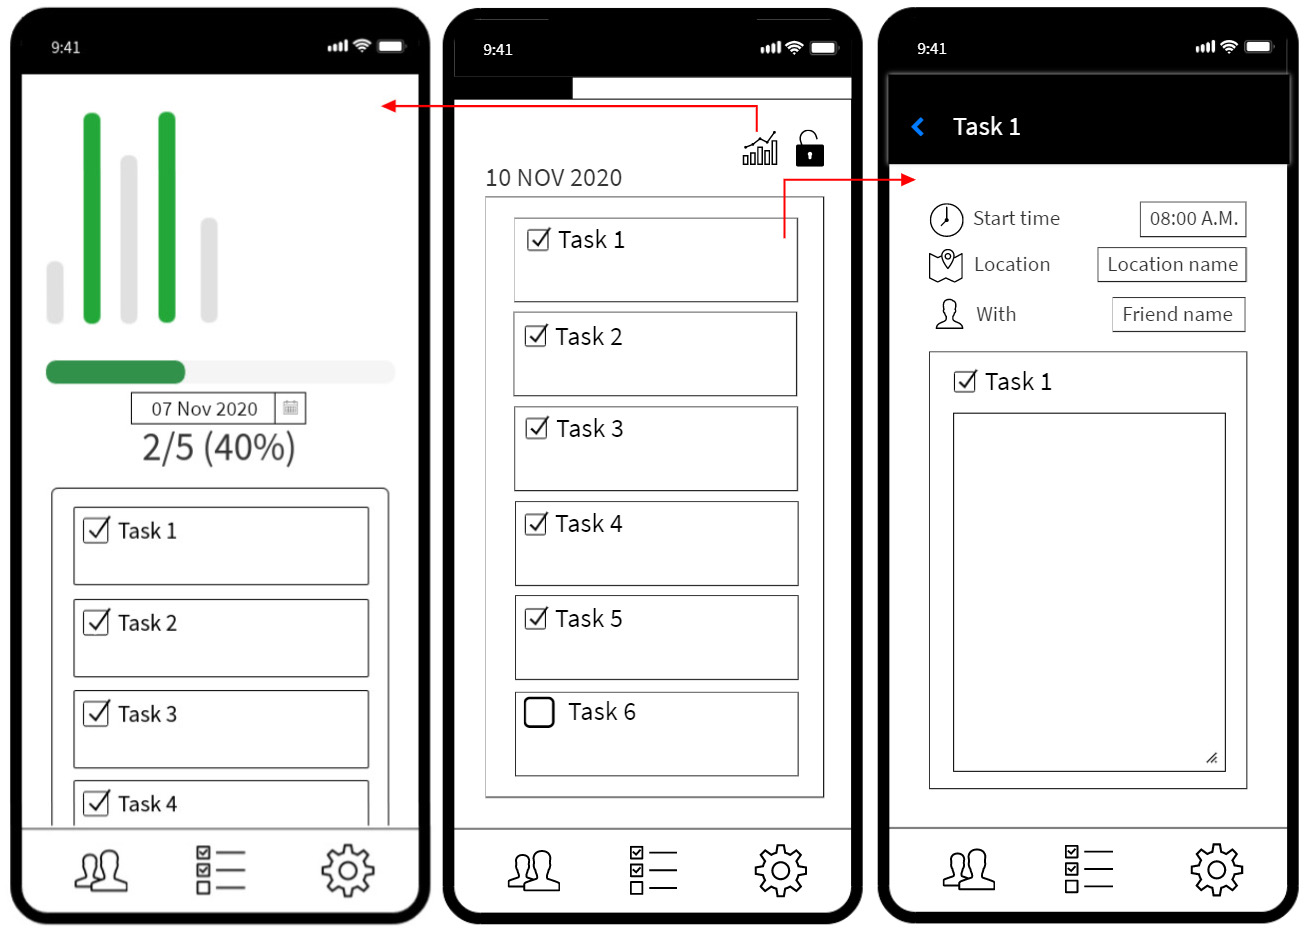
\includegraphics[width=270pt]{3) Tasks.jpg} \caption{Tasks (Main Screen)} \label{fig:Tasks} \end{figure}  
    
    \item Tasks (Main Screen): \\
    In main screen, authentication is required. Token should be stored in local storage and be used when calling API server service. User can click on the chart button to see their dashboard. Lock button on the right is a button to freeze the tasks and user can adjust the lock time in the settings. Details can be set when the user presses the tasks.
    \begin{enumerate}
        \item One task component: \\
        In a task component, there are details of a specific task. For showing the detail, API call is required. And in application, there is global store for saving data state. All the data is stored in one global Redux store, and it is only updated by dispatch function.
    \begin{lstlisting}[frame=single]
    # in Application
    data := apiCall(type, taskID)
    # CRUD API call
    dispatch(updateStore(data))
        .then(re-render())
    \end{lstlisting}
    
    \begin{lstlisting}[frame=single]
    # in API server
    type, taskID := request
    taskTable(where id = taskID)
        .action(type)
    # CRUD of task detail
    \end{lstlisting}
        \item Task list component: \\
        Task list component data is also managed by Redux store. All the API call and the result are being updated to the store through redux's dispatch function like above.

        \item Dashboard: \\
        The application should be able to get the log of user's usage by period. Data is stored in DynamoDB, so API call is required. And also the data is managed by redux.
    \begin{lstlisting}[frame=single]
    # in Application
    data := getLogOf["weekly"]()
    dispatch(updateDashboard(data))
        .then(re-render())
    \end{lstlisting}
\end{enumerate}
    
\begin{figure}[htp] \centering 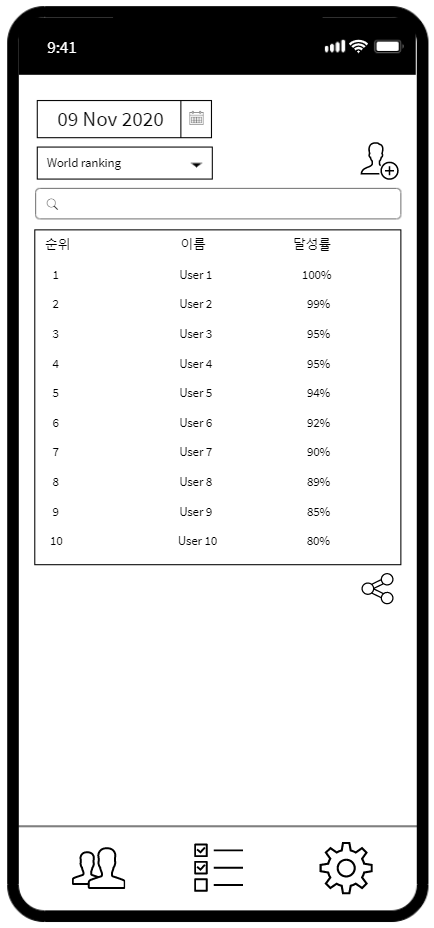
\includegraphics[width=120pt]{4) Social.PNG} \caption{Social} \label{fig:Social} \end{figure}
    
    \item Social: \\
    Friend list comes out when the user clicks the bottom social navigation tab. It shows the list of user's friends and at the same time, the ranking. Users can select to see the ranking of their friends or the world by pressing the ranking button. They can also add friends through the add button, and share the result through the share button. It is available to search the specific user, be friends and check the result of their six tasks.
    
\begin{figure}[htp] \centering 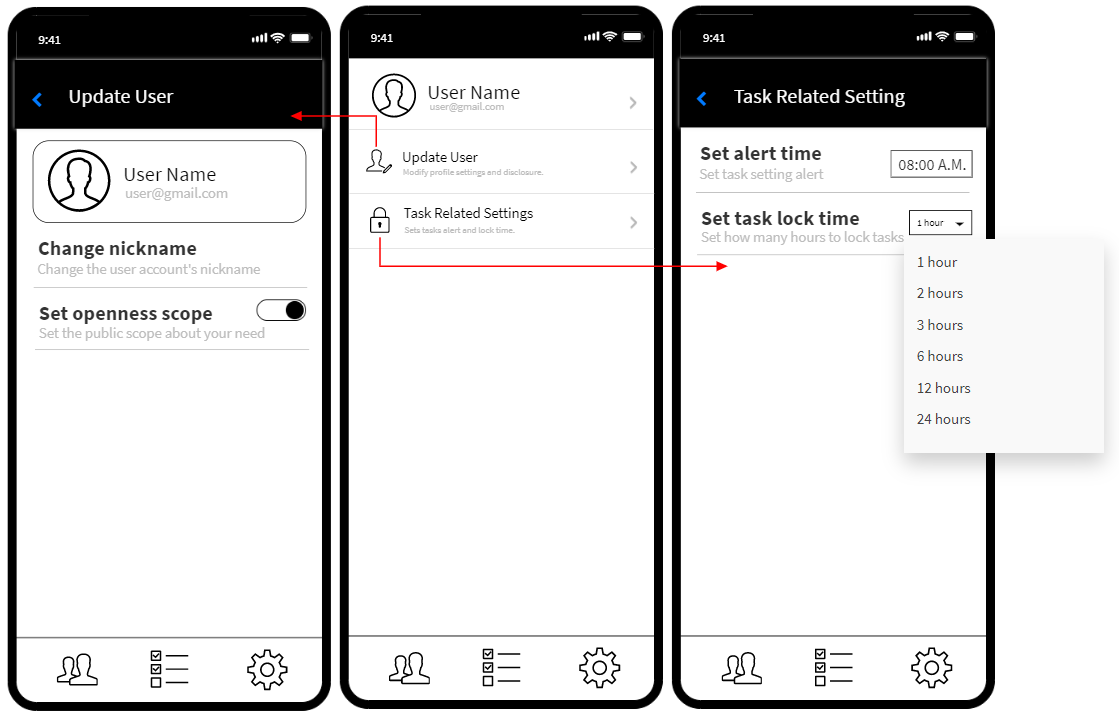
\includegraphics[width=300pt]{5) Settings.PNG} \caption{Settings} \label{fig:Settings} \end{figure}    
    
    \item Settings: \\
    In the settings screen, there are features about updating user information, and setting task related settings. Task related settings use local device's options. Alarm and task session time use device's timer API and updating user information uses API call.
    \begin{lstlisting}[frame=single]
    # lock session time
    default = 8 * HOUR
    lockSessionTime = default
    onUpdateSessionTime((time) => {
        lockSessionTime = time
    }})
    
    # alarm
    default = 3 * HOUR
    triggerTimer = default
    onUpdateTriggerTime((time) => {
        triggerTimer = time
    })
    
    # update user info
    apiCall(updateData)
    \end{lstlisting}

\end{enumerate}

\subsection{NUGU Service}

Every utterance command is sent to processing backend server through NUGU SDK. NUGU SDK processes the voice to string. And backend proxy server changes the string to valid command form and send it to the api server.

\begin{lstlisting}[frame=single]
voice > NUGU SDK > Processed voice string
> Backend Proxy server > API Server
\end{lstlisting}

\end{document}
